\documentclass{article}

\usepackage[a4paper,margin=2cm]{geometry}
\usepackage{soul, color}
\usepackage{graphicx}
\usepackage{hyperref}

\title{COMP30024 Assignment 1 - Report}
\date{\today}
\author{Lucas Fern (1080613),\\Hugo Lyons Keenan (1081696)}

\begin{document}
\maketitle
\subsection*{How did you formulate this game as a search problem? Explain your view of the problem in terms of states, actions, goal tests, and path costs, as relevant.}
The game was thought of as a tree of board states, with the root node as the initial game state and children of each node being all board states reachable by legal moves. In this model, states are individual board states and actions are complete sets of moves that ‘upper’ can take to enter a new state (complete sets involve moving all pieces). In traversing the tree, path cost is thought of as the number of moves though board-state space to get from one state to another - this is equivalent to the number of walks down branches of the tree. The win condition is met when all lower tokens have been defeated, this is the goal test. 

\subsection*{What search algorithm does your program use to solve this problem, and why did you choose this algorithm? Comment on the algorithm’s efficiency, completeness, and optimality. If you have developed heuristics to inform your search, explain them and comment on their admissibility.}
The program uses the A* algorithm to determine the most favourable actions. This search algorithm was chosen as it is complete for problems with finite state spaces like RoPaSci360, as well as being optimal when provided a consistently admissible heuristic. A* uses a combined evaluation function: $f(n) = h(n) + g(n)$, where $g(n)$ is the cost to get from the starting node to node $n$ (known) and $h$ is the estimated cost to get from node $n$ to the goal node. In choosing a heuristic function, $h(n)$, we considered admissible heuristics such as \textit{half of the average hexagonal Manhattan distance between each lower token and its closest predator}\footnote{A token's predator is the piece on the opposite team which can kill it. eg. $P$ is a predator of $r$} (see Figure \ref{fig: hex manhattan},) but after comparing the speed of a variety of heuristics, and considering there was no constraint on finding an optimal solution, an inadmissible heuristic was selected.\\[2mm]
The heuristic which was ultimately used was the sum of the distances between each lower token and it's closest predator \footnote{We also added an inconsequential amount of random noise to the heuristic to efficiently break ties between nodes in the search tree with equal heuristic values}. But rather than using the Hexagonal Manhattan Distance, a Breadth First Search \footnote{adapted from \url{https://www.redblobgames.com/pathfinding/a-star/introduction.html}} was used to find the length of a path which navigated around all blocked hexes on the board. This was a vastly superior estimate of the actual distance to a node in cases with many block tokens, and allowed us to find paths to the goal in situations where other choices of heuristic would get stuck unable to navigate an obstacle.\\[2mm]
It was a conscious decision that this heuristic is not admissible, in fact in almost every case it vastly overestimates the amount of turns remaining in the game. Although this means our algorithm cannot guarantee an optimal solution, profiling of the program showed such substantial improvements in the execution time that we considered this a reasonable trade-off. This conclusion agrees with analysis of the A* algorithm which states states that A* ``...can run faster...if $h(n)$ is sometimes greater than the cost of moving from $n$ to the goal.''\footnote{From lectures Week 3: Informed Search Methods}

\begin{figure}
    \centering
    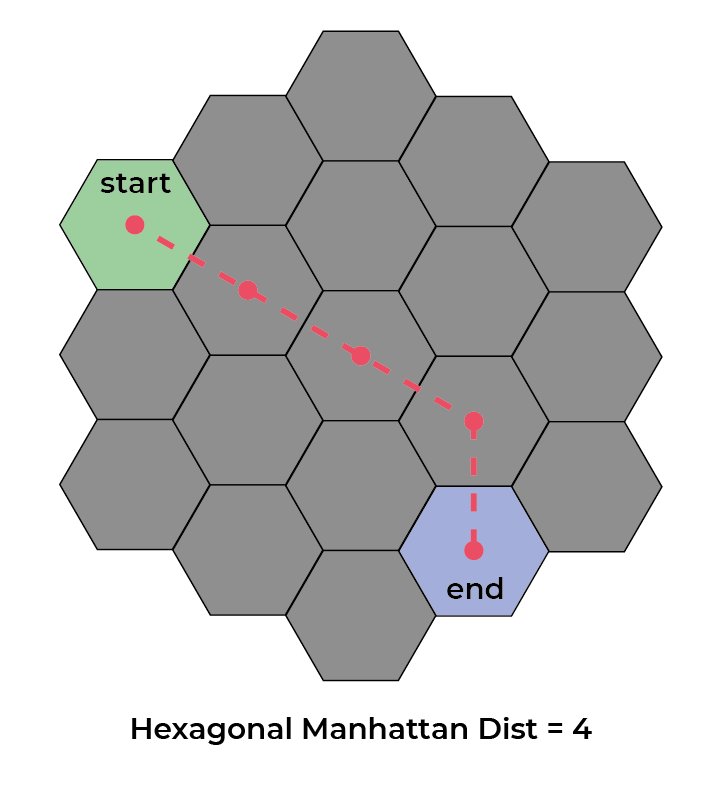
\includegraphics[width=0.4\textwidth]{hex-manhattan.png}
    \caption{A visualisation of the calculation of Hexagonal Manhattan Distance.}
    \label{fig: hex manhattan}
\end{figure}

\subsection*{How do the features of the starting configuration (the position and number of tokens) impact your program’s time and space requirements? For example, discuss their connection with the branching factor and search tree depth and how these affect the time and space complexity of your algorithm.}
\hl{The time complexity of the program is exponential in the product of error in $h(n)$ and the length of the solution set of moves.\footnote{can we make this clearer somehow? I'm not really sure what its saying myself, our fastest algorithm has huge error in $h(n)$}} This means that configurations with ‘obstacles’ between lower and their predator upper tokens, as well as configurations with predator upper tokens far away from their prey require more time. These also require more space, as each board state visited is stored in memory to make sure the algorithm does not back track, or get caught in loops. Additionally, as the number of upper tokens in the starting configuration increases, the branching factor increases exponentially. This is because the number of possible actions from one board state is the number of terms in the cartesian product of the possible moves for each upper token. For example, with just one upper token the maximum number of actions is 6. With two it is 36, without even considering swing actions. This means that solutions for configurations with many upper tokens can be more resource intensive to find. Additionally, although the impact of lower tokens is not as great as upper tokens, having many can cause the solution to be very long, further increasing run time and space requirements.
\end{document}